\documentclass[9pt,a4paper]{extarticle}

\usepackage[a4paper,margin=16mm]{geometry}
\usepackage{amsmath,amssymb,mathtools}
\usepackage{booktabs,tabularx,array}
\usepackage{microtype}
\usepackage{tikz}
\usetikzlibrary{arrows.meta,calc,fit,positioning,shapes.geometric}
\usepackage{xcolor}
\usepackage[hidelinks]{hyperref}

\definecolor{elastic}{HTML}{D97745}
\definecolor{elasticlight}{HTML}{F9E6DA}
\definecolor{plastic}{HTML}{3C7196}
\definecolor{plasticlight}{HTML}{DFEBF3}
\definecolor{good}{HTML}{4D8562}
\definecolor{goodlight}{HTML}{E2F0E6}
\definecolor{bad}{HTML}{A44942}
\definecolor{badlight}{HTML}{F5E1DF}
\definecolor{ink}{HTML}{28343D}
\definecolor{muted}{HTML}{66737C}
\definecolor{panel}{HTML}{F3F5F6}

\newcommand{\Fminus}{F^-}
\newcommand{\Fplus}{F^+}
\newcommand{\Em}{F_E^-}
\newcommand{\Ep}{F_E^+}
\newcommand{\Pm}{F_P^-}
\newcommand{\Pp}{F_P^+}
\newcommand{\Hf}{H_{\mathcal F}}
\newcommand{\Hp}{H_P}
\newcommand{\Ttot}{T_{\mathrm{total}}}

\setlength{\parindent}{0pt}
\setlength{\parskip}{0.38em}
\setlength{\tabcolsep}{5pt}
\pagestyle{plain}

\tikzset{
  >=Latex,
  matrixbox/.style={draw,rounded corners=2pt,inner sep=5pt,align=center},
  flowbox/.style={draw=ink,rounded corners=2pt,inner sep=6pt,align=center,
                  text width=30mm},
  smallflow/.style={draw=ink,rounded corners=2pt,inner sep=5pt,align=center,
                    text width=25mm},
  arrow/.style={->,line width=0.75pt,draw=muted},
  nodept/.style={circle,fill=ink,inner sep=1.6pt}
}

\begin{document}

\begin{center}
  {\LARGE\bfseries What should reconnection remember?}\\[0.3em]
  {\large Plastic well changes must persist; elastic remeshing changes must not}
\end{center}

\begin{center}
\begin{minipage}{0.94\linewidth}
\colorbox{panel}{%
\parbox{0.95\linewidth}{%
\textbf{Result.}
An edge flip changes both the local element and its square reference.  The
plastic part of this change identifies which lattice well the element has
reached and should be stored.  The accompanying change in elastic deformation
belongs to the old parent-child geometry and must remain recoverable.  If the
full gradient is made exactly invariant, this elastic mismatch is frozen into
$\Hf$.  A later square element can then be reported as elastically strained.
The plastic-history construction avoids this: every square geometry is mapped
to a square-lattice ground state, while the accumulated plastic well is still
remembered.}}
\end{minipage}
\end{center}

\section{One edge flip is enough}

The example uses the pre-flip deformation gradient
\begin{equation}
\Fminus=
\begin{pmatrix}1&1\\0.6&1.6\end{pmatrix}.
\label{eq:Fminus}
\end{equation}
It can occur in a four-node edge flip for which the descendant associated with
this parent is a square triangle after reconnection.  Thus the example takes
\begin{equation}
\Fplus=I.
\label{eq:Fplus}
\end{equation}
Figure~\ref{fig:flip} shows one compatible geometry.  The important point is
not the particular node positions, but that the parent and child have different
elastic parts even though the child is a local energy minimum.

\begin{figure}[h]
\centering
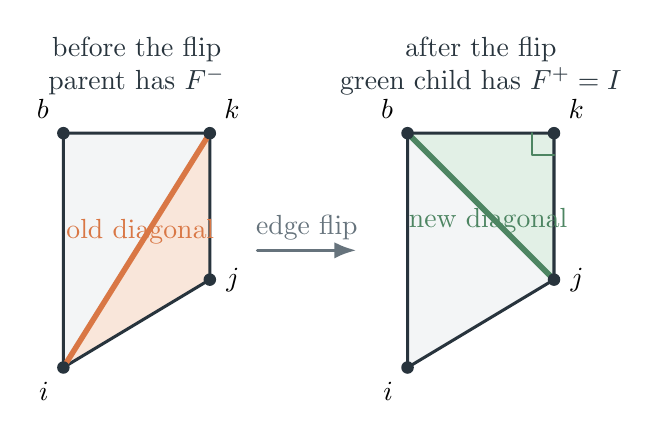
\begin{tikzpicture}[scale=0.93,line cap=round,line join=round]
  % Before
  \begin{scope}[xshift=0cm]
    \coordinate (i) at (0,0);
    \coordinate (j) at (2,1.2);
    \coordinate (k) at (2,3.2);
    \coordinate (b) at (0,3.2);
    \fill[elasticlight] (i)--(j)--(k)--cycle;
    \fill[panel] (i)--(k)--(b)--cycle;
    \draw[ink,line width=1.1pt] (i)--(j)--(k)--(b)--cycle;
    \draw[elastic,line width=2.0pt] (i)--(k);
    \node[nodept,label=below left:$i$] at (i) {};
    \node[nodept,label=right:$j$] at (j) {};
    \node[nodept,label=above right:$k$] at (k) {};
    \node[nodept,label=above left:$b$] at (b) {};
    \node[align=center,text=ink] at (1,4.12)
      {before the flip\\parent has $\Fminus$};
    \node[align=center,text=elastic] at (1.05,1.85)
      {old diagonal};
  \end{scope}

  \draw[arrow,line width=1.1pt] (2.65,1.6)--(4.0,1.6)
    node[midway,above,text=muted]{edge flip};

  % After
  \begin{scope}[xshift=4.7cm]
    \coordinate (i) at (0,0);
    \coordinate (j) at (2,1.2);
    \coordinate (k) at (2,3.2);
    \coordinate (b) at (0,3.2);
    \fill[panel] (i)--(j)--(b)--cycle;
    \fill[goodlight] (j)--(k)--(b)--cycle;
    \draw[ink,line width=1.1pt] (i)--(j)--(k)--(b)--cycle;
    \draw[good,line width=2.0pt] (j)--(b);
    \node[nodept,label=below left:$i$] at (i) {};
    \node[nodept,label=right:$j$] at (j) {};
    \node[nodept,label=above right:$k$] at (k) {};
    \node[nodept,label=above left:$b$] at (b) {};
    \draw[good,line width=0.8pt] ($(k)+(-0.30,0)$)--
      ($(k)+(-0.30,-0.30)$)--($(k)+(0,-0.30)$);
    \node[align=center,text=ink] at (1,4.12)
      {after the flip\\green child has $\Fplus=I$};
    \node[align=center,text=good] at (1.1,2.0)
      {new diagonal};
  \end{scope}
\end{tikzpicture}
\caption{A single asymmetric edge flip.  The old highlighted parent is
distorted; the associated new child is an exact square reference triangle.
The new child should therefore be recognized as a local energy minimum.}
\label{fig:flip}
\end{figure}

\section{What is elastic, and what is plastic?}

Square-lattice reduction gives the exact multiplicative decomposition
\begin{equation}
\Fminus=
\underbrace{\begin{pmatrix}1&0\\-0.4&1\end{pmatrix}}_{\displaystyle \Em}
\underbrace{\begin{pmatrix}1&1\\1&2\end{pmatrix}}_{\displaystyle \Pm}.
\label{eq:decomp}
\end{equation}
The first factor is a recoverable vertical shear.  The second is an integer
unimodular lattice transformation:
\begin{equation}
\Pm=
\begin{pmatrix}1&0\\1&1\end{pmatrix}
\begin{pmatrix}1&1\\0&1\end{pmatrix}
=:V_1H_1,
\qquad
\substack{V_1:\ \text{one vertical slip}\\
           H_1:\ \text{one horizontal slip}.}
\label{eq:plastic}
\end{equation}
Thus both histories should remember that the element has moved to another
lattice well.  They differ only in whether the old elastic shear is also made
permanent.

\begin{figure}[h]
\centering
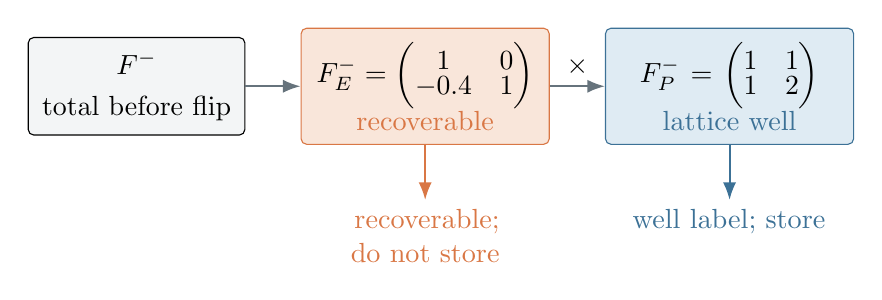
\begin{tikzpicture}[node distance=5mm and 7mm]
  \node[matrixbox,fill=panel,text width=24mm] (F)
    {$\displaystyle \Fminus$\\[1mm] total before flip};
  \node[matrixbox,fill=elasticlight,draw=elastic,text width=28mm,right=of F] (E)
    {$\displaystyle \Em=\begin{pmatrix}1&0\\[-1mm]-0.4&1\end{pmatrix}$\\
     \textcolor{elastic}{recoverable}};
  \node[matrixbox,fill=plasticlight,draw=plastic,text width=28mm,right=of E] (P)
    {$\displaystyle \Pm=\begin{pmatrix}1&1\\[-1mm]1&2\end{pmatrix}$\\
     \textcolor{plastic}{lattice well}};
  \draw[arrow] (F)--(E);
  \draw[arrow] (E)--(P) node[midway,above]{$\times$};

  \node[align=center,text=elastic,text width=29mm,below=7mm of E] (change)
    {recoverable; do not store};
  \node[align=center,text=plastic,text width=29mm,below=7mm of P] (store)
    {well label; store};
  \draw[arrow,draw=elastic] (E)--(change);
  \draw[arrow,draw=plastic] (P)--(store);
\end{tikzpicture}
\caption{The physical division of responsibility.  Elastic deformation is
recoverable state; the plastic factor labels the lattice well.  Reconnection
history should store the blue factor, not the orange one.}
\label{fig:parts}
\end{figure}

\section{What each history stores}

Let both histories initially equal $I$.  Direct invariance of the full gradient
uses
\begin{equation}
\Hf^+=(\Fplus)^{-1}\Fminus\Hf^-,
\qquad \mathcal F=F\Hf.
\label{eq:direct}
\end{equation}
Since $\Fplus=I$, this writes the entire old gradient into memory:
\begin{equation}
\boxed{\Hf^+=\Em\Pm.}
\label{eq:directmemory}
\end{equation}
The plastic-history rule instead uses
\begin{equation}
\Hp^+=(\Pp)^{-1}\Pm\Hp^-,
\qquad \Ttot=F\Hp.
\label{eq:plasticupdate}
\end{equation}
The square child has $\Pp=I$, so only the well change is stored:
\begin{equation}
\boxed{\Hp^+=\Pm.}
\label{eq:plasticmemory}
\end{equation}

\begin{figure}[h]
\centering
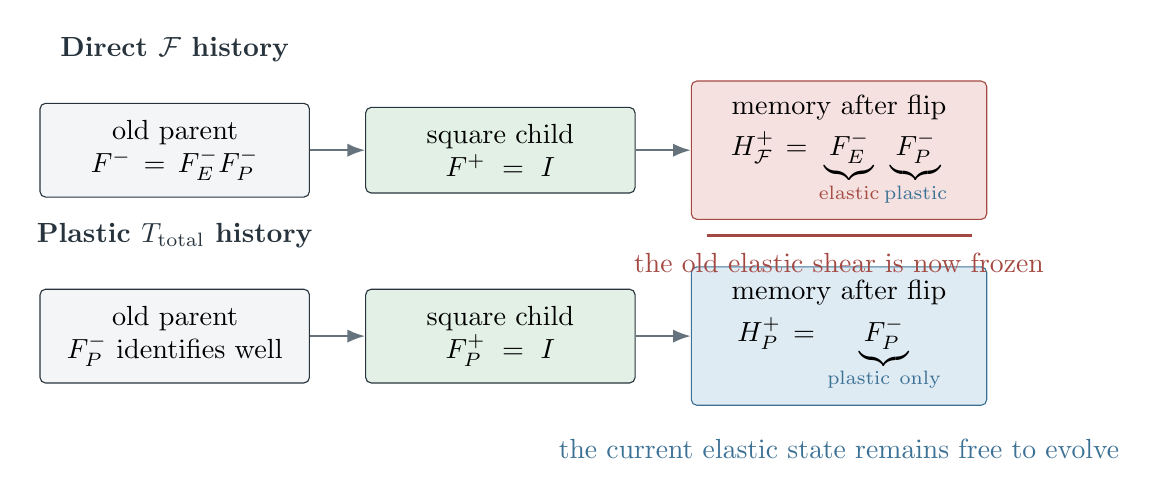
\begin{tikzpicture}[node distance=7mm and 7mm]
  % headings
  \node[align=center,text=ink,font=\bfseries] (directtitle)
    {Direct $\mathcal F$ history};
  \node[flowbox,fill=panel,below=4mm of directtitle] (directold)
    {old parent\\$\Fminus=\Em\Pm$};
  \node[flowbox,fill=goodlight,right=of directold] (directnew)
    {square child\\$\Fplus=I$};
  \node[matrixbox,fill=badlight,draw=bad,text width=34mm,right=of directnew] (directmem)
    {memory after flip\\[1mm]
     $\Hf^+=\underbrace{\Em}_{\textcolor{bad}{\text{elastic}}}
                   \underbrace{\Pm}_{\textcolor{plastic}{\text{plastic}}}$};
  \draw[arrow] (directold)--(directnew);
  \draw[arrow] (directnew)--(directmem);

  \node[align=center,text=ink,font=\bfseries,below=18mm of directtitle] (plastictitle)
    {Plastic $T_{\mathrm{total}}$ history};
  \node[flowbox,fill=panel,below=4mm of plastictitle] (plasticold)
    {old parent\\$\Pm$ identifies well};
  \node[flowbox,fill=goodlight,right=of plasticold] (plasticnew)
    {square child\\$\Pp=I$};
  \node[matrixbox,fill=plasticlight,draw=plastic,text width=34mm,right=of plasticnew] (plasticmem)
    {memory after flip\\[1mm]
     $\Hp^+=\underbrace{\Pm}_{\textcolor{plastic}{\text{plastic only}}}$};
  \draw[arrow] (plasticold)--(plasticnew);
  \draw[arrow] (plasticnew)--(plasticmem);

  \draw[bad,line width=0.9pt] ($(directmem.south west)+(2mm,-2mm)$)--
    ($(directmem.south east)+(-2mm,-2mm)$);
  \node[below=3mm of directmem,align=center,text=bad]
    {the old elastic shear is now frozen};
  \node[below=3mm of plasticmem,align=center,text=plastic]
    {the current elastic state remains free to evolve};
\end{tikzpicture}
\caption{The decisive difference is the content of memory.  Both methods
remember $\Pm$; only the direct history also stores the elastic parent-child
mismatch.}
\label{fig:memory}
\end{figure}

The example $\Fplus=I$ makes the mechanism transparent.  For a general flip,
write
\[
\Fminus=\Em\Pm,
\qquad
\Fplus=\Ep\Pp.
\]
Then
\begin{align}
\Hf^+&=(\Pp)^{-1}\underbrace{(\Ep)^{-1}\Em}_{
\text{elastic parent-child mismatch}}\Pm\Hf^-,
\label{eq:generaldirect}\\
\Hp^+&=(\Pp)^{-1}\Pm\Hp^-.
\label{eq:generalplastic}
\end{align}
Equation~\eqref{eq:generaldirect} shows exactly where the unwanted elastic
information enters.  If $\Ep=\Em$, the mismatch is $I$ and the methods agree.
If the elastic component changes during remeshing, one flip is sufficient to
separate them.

\section{Return to a square geometry}

Now consider the descendant at any later time when its current local geometry
is again a square triangle, so $F=I$.  This is a local minimum of the actual
element energy.  The two reconstructions are
\begin{align}
\mathcal F_{\square}
 &=I\Hf^+=\Em\Pm,
\label{eq:finaldirect}\\
(\Ttot)_{\square}
 &=I\Hp^+=\Pm.
\label{eq:finalplastic}
\end{align}

\begin{figure}[h]
\centering
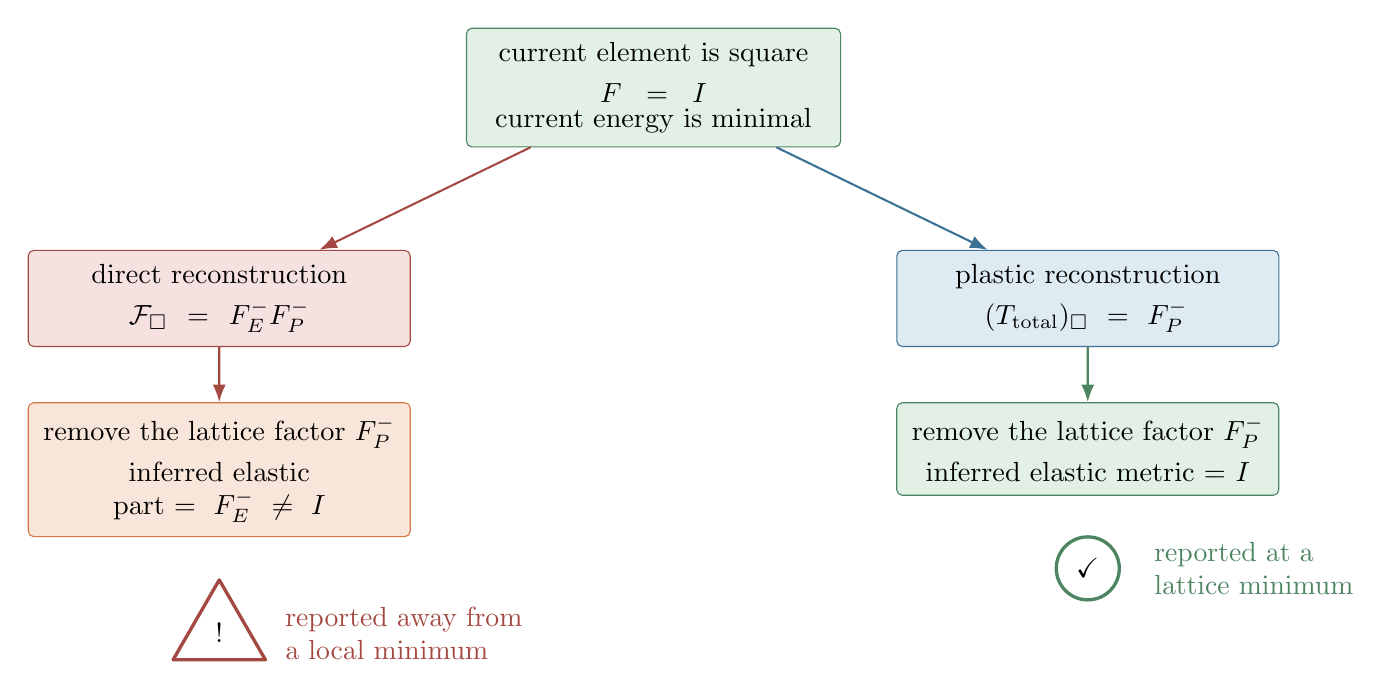
\begin{tikzpicture}[scale=0.88,line cap=round,line join=round]
  % Shared input
  \node[matrixbox,fill=goodlight,draw=good,text width=44mm] (square)
    {current element is square\\[1mm]
     $F=I$\\[-1mm]
     current energy is minimal};

  % Direct branch
  \node[matrixbox,fill=badlight,draw=bad,text width=45mm,
        below left=13mm and 7mm of square] (badstate)
    {direct reconstruction\\[1mm]
     $\mathcal F_{\square}=\Em\Pm$};
  \node[matrixbox,fill=elasticlight,draw=elastic,text width=45mm,
        below=7mm of badstate] (badreduce)
    {remove the lattice factor $\Pm$\\[1mm]
     inferred elastic part $=\Em\ne I$};
  \node[draw=bad,very thick,regular polygon,regular polygon sides=3,
        minimum size=8mm,below=5mm of badreduce] (warn) {!};
  \node[right=3mm of warn,align=left,text=bad]
    {reported away from\\a local minimum};

  % Plastic branch
  \node[matrixbox,fill=plasticlight,draw=plastic,text width=45mm,
        below right=13mm and 7mm of square] (goodstate)
    {plastic reconstruction\\[1mm]
     $(\Ttot)_{\square}=\Pm$};
  \node[matrixbox,fill=goodlight,draw=good,text width=45mm,
        below=7mm of goodstate] (goodreduce)
    {remove the lattice factor $\Pm$\\[1mm]
     inferred elastic metric $=I$};
  \node[draw=good,very thick,circle,minimum size=8mm,
        below=5mm of goodreduce] (check) {$\checkmark$};
  \node[right=3mm of check,align=left,text=good]
    {reported at a\\lattice minimum};

  \draw[arrow,draw=bad] (square)--(badstate);
  \draw[arrow,draw=plastic] (square)--(goodstate);
  \draw[arrow,draw=bad] (badstate)--(badreduce);
  \draw[arrow,draw=good] (goodstate)--(goodreduce);
\end{tikzpicture}
\caption{The same square current geometry receives two different
interpretations.  The plastic history retains the correct well while allowing
the elastic state to return to a minimum.  Direct invariance leaves the old
elastic shear embedded in the reconstructed gradient.}
\label{fig:return}
\end{figure}

The plastic result is not literally the matrix $I$ because it correctly
remembers one vertical and one horizontal slip.  It is nevertheless a
square-lattice ground state: after lattice reduction its elastic metric is
$I$.  By contrast, reducing $\mathcal F_{\square}$ removes $\Pm$ but leaves
\begin{equation}
\Em=\begin{pmatrix}1&0\\-0.4&1\end{pmatrix},
\qquad
(\Em)^T\Em=
\begin{pmatrix}1.16&-0.4\\-0.4&1\end{pmatrix}\ne I.
\label{eq:residual}
\end{equation}
Thus $\mathcal F$ would describe a non-minimal elastic state even though the
current nodes form a minimal-energy square triangle.

\section{Interpretation and recommendation}

\begin{center}
\renewcommand{\arraystretch}{1.17}
\begin{tabularx}{0.96\linewidth}{@{}>{\raggedright\arraybackslash}p{0.28\linewidth}
  >{\raggedright\arraybackslash}X >{\raggedright\arraybackslash}X@{}}
\toprule
 & \textbf{Direct $\mathcal F$ history} & \textbf{Plastic $\Ttot$ history}\\
\midrule
What survives a flip
  & Plastic well plus elastic parent-child mismatch
  & Plastic well only\\
What remains free to recover
  & Only deformation occurring after the mismatch was stored
  & The complete current elastic component\\
Square current geometry
  & Can be reported outside the local energy minimum
  & Always maps to a square-lattice ground state\\
What is remembered correctly
  & Exact algebraic invariance of the inherited full parent gradient
  & The accumulated sequence of lattice slips\\
Appropriate interpretation
  & A record of an imposed parent-child correspondence, not a reliable current elastic state
  & Reconnection-invariant plastic history combined with the current elastic state\\
\bottomrule
\end{tabularx}
\end{center}

The history variable is an approximation necessitated by reconnecting; it does
not define the simulation forces.  Its physically useful role is therefore to
remember information that the current geometry cannot recover on its own.  The
current geometry already determines the elastic deformation.  What it loses at
an edge flip is the discrete lattice-well label.

Consequently, the history should preserve $F_P$ but not the change in $F_E$.
The recommended reconstructed measure is
\begin{equation}
\boxed{
T=F_P\Hp,
\qquad
\Ttot=F_E T=F\Hp,
\qquad
\Hp^+=(\Pp)^{-1}\Pm\Hp^- .}
\end{equation}
This construction remembers every plastic well change while ensuring that a
minimal-energy current geometry is always represented by a minimal-energy
deformation gradient.

\end{document}
